\documentclass[11pt]{article}
\usepackage[utf8]{inputenc}
\usepackage[T1]{fontenc}
\usepackage{lmodern}
\usepackage{microtype}
\usepackage[margin=1in]{geometry}
\usepackage{graphicx}
\usepackage{booktabs}
\usepackage{amsmath,amssymb}
\usepackage{xcolor}
\usepackage{hyperref}
\usepackage{enumitem}
\usepackage{listings}
\hypersetup{colorlinks=true, linkcolor=blue!50!black, urlcolor=blue!50!black}
\lstset{basicstyle=\ttfamily\small, columns=fullflexible, keepspaces=true, frame=single,
  framerule=0.3pt, rulecolor=\color{black!30}, xleftmargin=4pt, xrightmargin=4pt, aboveskip=8pt,
  belowskip=8pt, showstringspaces=false, literate={θ}{{$\theta$}}1 {ν}{{$\nu$}}1 {κ}{{$\kappa$}}1}
\setlist{itemsep=2pt, topsep=4pt}

\title{\textbf{The Mechanism Layer in \texttt{cdm} v0.3}\\[4pt]
\large Novelty and feasibility of how an option works}
\author{Chris Kagabe \& Archymedes}
\date{October 2026}

\begin{document}
\maketitle

\begin{abstract}
\noindent This document describes the mechanism layer added to \texttt{cdm} in version 0.3: what
it computes, how it changes decisions, how to use it, and the evidence for and against it. The
layer describes each option by the functions it must perform and the working principle it uses for
each. Novelty is computed from that description instead of from a judged score, an unproven working
principle is sent to a prototype test instead of being vetoed, and the outcome of each test updates
a belief that is shared by every option using the same principle. Full derivations are in the paper,
\emph{Unknown Is Not Risky} (v0.3.0), \S5 and Appendix~A.
\end{abstract}

\section{Purpose}

Version 0.2 decided which options were novel with one ordinal question to the judge (``how
different is the approach from every precedent?''). This had two consequences.
\begin{enumerate}
\item The score depends on how an option is written. On Jev, describing the same mechanism with
promotional wording raised the score by $0.058$ on a $[0,1]$ scale.
\item The score does not identify a mechanism. A check of one option therefore produced no
information about any other option, even one built on the same idea.
\end{enumerate}
Engineering design addresses both by describing a solution as a set of \emph{functions}, each
performed by a \emph{working principle} (the morphological chart of Zwicky; the function structures
of Pahl and Beitz). The mechanism layer adopts that description. Novelty and feasibility become
properties of principles, and principles are shared across options and across decisions.

\section{Concepts}

\begin{description}[leftmargin=0pt]
\item[Function.] A result the solution must achieve, for example ``collect the monthly fee''. Each
function has a weight $w_f$ and a catalogue of known working principles.
\item[Working principle.] A way of achieving a function, for example ``cash collected on a visit''
or ``mobile money''. A principle outside the catalogue is labelled \textsc{new}.
\item[Record.] The precedents: for each, which principle it used for each function. The record
defines what counts as familiar.
\item[Classification $\pi_{i,f}$.] The judge's distribution over the catalogue plus \textsc{new}
for option $i$ and function $f$, asked as a Choice question over all cyclic orderings so that
position bias cancels.
\item[Risk estimate $r_{i,f}$.] The judge's probability that the way option $i$ performs $f$ fails
in this setting (a Noul question).
\end{description}

\section{Quantities}

\begin{table}[h]
\centering\small
\setlength{\tabcolsep}{4pt}
\begin{tabular}{@{}p{0.19\linewidth}p{0.42\linewidth}p{0.35\linewidth}@{}}
\toprule
quantity & definition & meaning \\
\midrule
principle novelty & $N_f(p)=1-\min(1,c_{f,p}/m_f)$; $N_f(\textsc{new})=1$ & 1 if no precedent used $p$ for $f$ (default $m_f=1$) \\
mechanism novelty & $\nu_i=\sum_f\bar w_f\sum_p\pi_{i,f}(p)N_f(p)$ & weighted probability of an unused principle \\
combination novelty & $\kappa_i=1-\sum_{r\in R^\ast}\prod_f\pi_{i,f}(r_f)$ & probability the combination is in no precedent \\
reliability belief & $\bar\theta_{f,p}$ (see below) & probability that $p$ performs $f$ here \\
mechanism risk & $q_i^{\mathrm{mech}}=1-\prod_f\sum_p\pi_{i,f}(p)\bar\theta_{i,f,p}$ & probability the mechanism fails \\
learning value & $\Lambda_i=\sum_f\sum_p\pi_{i,f}(p)\,\bar\theta(1-\bar\theta)/(n+1)$ & what a test of the option would teach \\
\bottomrule
\end{tabular}
\end{table}

\noindent The reliability belief for a principle comes from the first applicable source:
\begin{enumerate}
\item \emph{Evidence}: a $\mathrm{Beta}(a,b)$ built from test reports about that principle, shared by
all options that use it.
\item \emph{Settled}: probability 1 if a precedent in this setting used the principle for the
function and no test has contradicted it.
\item \emph{Opinion}: $\mathrm{Beta}(2(1-r_{i,f}),\,2r_{i,f})$, the judge's estimate held as two
pseudo-observations.
\end{enumerate}

\section{Effect on decisions}

The layer changes the policy in three places and leaves everything else unchanged.
\begin{enumerate}
\item \textbf{Innovation slot eligibility.} $\nu_i$ replaces the judged novelty, with its own gate
$\nu_{\min}=\tfrac12\min_f\bar w_f$ ($0.25$ for two equally weighted functions): the midpoint between
a repeated mechanism ($\nu=0$) and one unused principle in the lightest function. A reworded precedent
has $\nu=0$ and cannot take the slot. Override with \texttt{Policy(min\_mechanism\_novelty=...)}.
\item \textbf{Prototype gate.} $q_i^{\mathrm{mech}}$ is added as a hard constraint. An option built
on an untested principle has $q^{\mathrm{mech}}$ near $1/2$ and is placed in the \emph{verify}
state: it is tested, with a fallback to the status quo if the test fails. Evidence of failure
raises $q^{\mathrm{mech}}$ until the option is rejected.
\item \textbf{Optional learning bonus.} With \texttt{Policy(learning\_weight=w)}, the innovation slot
ranks options by $\mathrm{EI}_i+w\Lambda_i$. The default is $w=0$.
\end{enumerate}
Commit, portfolio, $P(\mathrm{best})$ and EVPI are computed as before. The axioms P1--P8 of the
policy continue to hold, because novelty and the learning bonus enter only the innovation slot.

\section{The value of a test across decisions}

For a single decision, only the mean of the belief about a violation matters (paper,
Proposition~1). Across decisions the spread matters. For a principle with belief
$\mathrm{Beta}(a,b)$, $n=a+b$, $\bar\theta=a/n$, and a later decision that gains
$\alpha(\mathbb E[\theta]-t)$ when it acts:
\[
\mathrm{VOI}(t)\;\le\;\alpha\,\frac{\bar\theta(1-\bar\theta)}{n+1},
\]
with equality at $t=\bar\theta$, and $\mathrm{VOI}(t)=0$ outside an interval of width $1/(n+1)$.
A principle with no evidence ($\mathrm{Beta}(1,1)$) is worth $101/3\approx34$ times as much to test
as one whose reliability is known to be one half ($\mathrm{Beta}(50,50)$).

\begin{figure}[h]
\centering
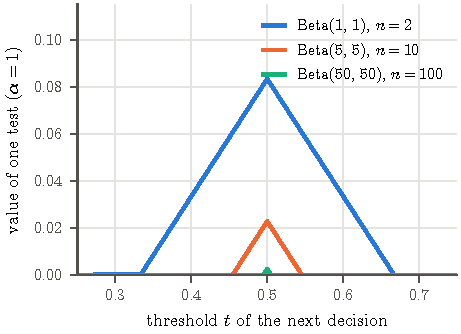
\includegraphics[width=0.5\linewidth]{../paper_figs/fig_mech_voi}
\caption{Value of one test for a later decision with threshold $t$, for three beliefs with mean
$0.5$.}
\end{figure}

\section{Usage}

\begin{lstlisting}[language=Python]
from cdm import (Function, JevJudge, Morphology, Policy, Problem,
                 decide, judge_problem)

reach = Function("reach", "find shop owners and convince them to sign up", {
    "door": "Staff visit shops in person",
    "referral": "Owners are rewarded for bringing in other owners"})
pay = Function("pay", "collect the monthly fee from shops", {
    "cash": "Cash collected during a visit",
    "momo": "Payment from the owner's mobile-money wallet"})
morph = Morphology([reach, pay], record=[{"reach": "door", "pay": "cash"}])

problem = Problem(goal=..., context=..., options=[...],
                  dimensions=[...], morphology=morph)
# the judge is asked the mechanism questions as well
judgments = await judge_problem(problem, [JevJudge()])
# the mechanism check is applied inside decide
decision = decide(problem, judgments, Policy())

# record a prototype test of mobile money once;
# every option that uses it is re-priced
morph.update("pay", "momo", passed=False, sens=0.9, spec=0.95)
\end{lstlisting}

\noindent Each \texttt{OptionStats} reports \texttt{novelty} ($\nu$), \texttt{combination}
($\kappa$), \texttt{learning} ($\Lambda$) and, among \texttt{checks}, \texttt{"mechanism"} when a
prototype test is required. Shah's rarity metric is available by passing
\texttt{familiar\_after=None} to \texttt{Morphology}.

\section{Evidence}

Five experiments test the layer; the paper (\S6.7--6.11) gives the details. Every number below is
checked against the result files by \texttt{scripts/verify\_figures.py}.

\begin{table}[h]
\centering\small
\setlength{\tabcolsep}{4pt}
\begin{tabular}{@{}p{0.2\linewidth}p{0.36\linewidth}p{0.38\linewidth}@{}}
\toprule
experiment & design & main result \\
\midrule
wording test (Jev) & 28 mechanisms, plain and hype & principle named in 111 of 112 cases; hype moves
judged novelty $+0.058$, $\nu$ $+0.005$ \\
disguise test (Jev) & 104 options: plain, hype, jargon, mundane & jargon on repeated mechanisms:
judged $+0.096$, $\nu$ $+0.043$; no wording changed an admission at the default gates \\
sequential benchmark & simulated, 24--48 related decisions, 300 worlds per setting & learning lowers
regret in every setting; late commitments to unreliable principles $26\%\to7\%$ \\
robustness sweep & one assumption varied at a time, 200 worlds & learning pays unless classification
is near chance; robust to interactions and catalogue size \\
Jev in the loop & Jev's real mechanism judgments, simulated outcomes, 1200 worlds & regret halved
against v0.2 ($-0.037$); ablation below \\
\bottomrule
\end{tabular}
\end{table}

\subsection*{Which part of the layer is useful}
The Jev-in-the-loop ablation splits the gain over v0.2 (regret $0.074$):
\begin{itemize}
\item \textbf{Novelty measure} ($\nu$ instead of the judged score): no gain ($-0.0003$). On Jev, the
judged novelty already separates repeated from new mechanisms; $\nu$ is better calibrated (error
$0.054$ against $0.128$) and moves less with wording, but this did not change decisions.
\item \textbf{Precedents as evidence} (the settled rule): $0.026$ $[0.023,0.028]$, with harm rising
from $3.3\%$ to $5.3\%$, because precedents' principles are deployed without a check.
\item \textbf{Learning per principle}: $0.012$ $[0.010,0.014]$ with the settled rule, $0.014$
$[0.011,0.016]$ without it, where it also lowers harm to $2.6\%$.
\item \textbf{Innovation pilot}: $0.0004$ $[-0.0006,0.0013]$, not measurable.
\end{itemize}
The layer is useful because naming principles lets evidence attach to them. Use learning per
principle; decide on the settled rule according to how reliable precedents' principles are; keep
the innovation pilot small or off.

\subsection*{When learning stops paying}
In the robustness sweep the regret reduction from learning was $0.0117$ with perfect classification,
$0.0076$ at $95\%$, $0.0033$ at $70\%$ and $0.0010$ (not significant) at $50\%$. With half of all
pairs of untested principles failing together, it was still $0.0064$. Jev classified $95$--$100\%$ of
cases correctly.

\section{Limits}

\begin{itemize}
\item The catalogue of principles is written by people. A poor catalogue produces poor novelty.
\item A principle filed under \textsc{new} accumulates no shared evidence until it is catalogued.
\item Principles are assumed not to interact, and classifications to be independent across
functions. $\kappa$ indicates where the first assumption matters most.
\item The settled rule treats a precedent in the same setting as proof that a principle works there.
\item The Jev tests use templated options. Outcomes in all sequential experiments are simulated
and share the model's structure; none establishes better decisions on real programmes.
\item The default gate on $\nu$ was introduced after the disguise test showed that the earlier gate
($0.5$) admitted only $56\%$ of new mechanisms; it is derived from the structure of $\nu$, not fitted.
\end{itemize}

\end{document}
